%%%%%%%%%% Prefix a "S" to all equations, figures, tables and reset the counter %%%%%%%%%%
\setcounter{equation}{0}
\setcounter{figure}{0}
\setcounter{table}{0}
\setcounter{page}{1}
\makeatletter

\renewcommand{\theequation}{S\arabic{equation}}
\renewcommand{\thefigure}{S\arabic{figure}}
%%%%%%%%%%%%%%%%%%%%

\subsection{1D Map in the immediate relaxation limit ($k\rightarrow\infty$) and its derivative} \label{supp: sub1}
We seek a function $\phi_{i+1}(\phi_i, b, \tau)$ describing the system's dynamics in the limit $k\rightarrow\infty$. Using the law of cosines and noting $\angle{rb}= \pi-\phi 2\pi$ (see Fig. \ref{osc}), the radial coordinate $r'(r,\phi,b)$ after perturbation is:
\begin{align}
    r'&=\sqrt{r^2+b^2-2rb\cos(\pi-\phi 2\pi)}\\
     &=\sqrt{r^2+b^2+2rb\cos(\phi 2\pi)} 
     \label{eq: r}.
\end{align}
Again, using the law of cosines, the angular coordinate $\phi'(r,\phi,b)$ after perturbation is $r =\sqrt{r'^2+b^2-2r'b\cos(\phi' 2\pi)}$. Then 
\begin{align}
    \cos(\phi' 2\pi) &= \frac{r^2+b^2+2rb\cos(\phi 2\pi) +b^2 - r^2}{2r'b} \\
    &= \frac{b+r \cos(\phi 2\pi)}{\sqrt{r^2+b^2+2rb\cos(\phi 2\pi)}} \\
    \phi' &= \frac{1}{2\pi}\arccos(\frac{b+r \cos(\phi 2\pi)}{\sqrt{r^2+b^2+2rb\cos(\phi 2\pi)}})
\end{align} where Eq. \ref{eq: r} is used in lines S3 and S4. However, $\arccos(\cos(2\pi \phi')) = 2\pi \phi'$ only if $0\leq \phi' \leq 1/2$. This is because arccosine only inverts the first half-period of cosine function between $0$ to $\pi$. For $1/2 \leq \phi' \leq 1$, we note that $-\arccos(\cos(2\pi \phi')) +2\pi= 2\pi \phi'$. So over the complete range of possible perturbed phases, we have:
\begin{equation}
    \phi' =
    \begin{cases}
     \frac{1}{2\pi}\arccos(\frac{b+r \cos(\phi 2\pi)}{\sqrt{r^2+b^2+2rb\cos(\phi 2\pi)}}) & 0 \leq \phi' \leq 1/2 \\
    -\frac{1}{2\pi}\arccos(\frac{b+r \cos(\phi 2\pi)}{\sqrt{r^2+b^2+2rb\cos(\phi 2\pi)}}) + 1 & 1/2 \leq \phi' \leq 1 \\
    \end{cases}.
\end{equation}
Integrating the angular differential equation is trivial: $\phi_{i+1} = \textnormal{mod} \{\phi'_i + \tau,1\}$ (see equation \ref{eqn:2}), which adds $\tau$ to the above piecewise equation. 
\begin{equation}
    \phi_{i+1} =
    \begin{cases}
     \frac{1}{2\pi}\arccos(\frac{b+r \cos(\phi 2\pi)}{\sqrt{r^2+b^2+2rb\cos(\phi 2\pi)}}) + \tau & 0 \leq \phi' \leq 1/2 \\
    -\frac{1}{2\pi}\arccos(\frac{b+r \cos(\phi 2\pi)}{\sqrt{r^2+b^2+2rb\cos(\phi 2\pi)}}) + 1 +\tau & 1/2 \leq \phi' \leq 1 \\
    \end{cases}
    \label{eq: b_plot}
\end{equation}
Note that since the perturbations are horizontal, if $0 \leq \phi \leq 1/2$, then $0 \leq \phi' \leq 1/2$; and if $1/2 \leq \phi \leq 1$, then $1/2 \leq \phi' \leq 1$ (i.e. the perturbation never causes the system to cross the x-axis). For $b<1$, as $\tau$ is increased from 0, the phase response curve ($\phi_{i+1}(\phi_i)$) intersects the line $\phi_{i+1}= \phi_i$ tangentially (see Figure \ref{b_plot}). Hence, we conclude that for $b<1$, the type of bifurcation for the period-1 instability boundary is a tangent bifurcation. 

\indent It is useful to rewrite $\phi_{i+1}(\phi_i,b,\tau)$ in a different form, which makes it easier to calculate the derivative $\frac{\partial \phi_{i+1}}{\partial \phi_i}$. We begin by noting that $\arccos(x) = \cot^{-1}(\frac{x}{\sqrt{1-x^2}})$ for $|x|<1$ which is always satisfied for any $\phi$, $b$, $r$, if $x=\frac{b+r \cos(\phi_i 2\pi)}{\sqrt{r^2+b^2+2rb\cos(\phi_i 2\pi)}}$. Then, 
\begin{align}
    \frac{x}{\sqrt{1-x^2}} &= \frac{b + \cos(2\pi \phi_i)}{\sin(2\pi \phi_i)} & r_i = 1 \nonumber \\
    &= b\csc(2\pi \phi_i) + \cot(2\pi \phi_i)
\end{align} 
Which allows us to simplify the 1D map to,
\begin{equation}
    \phi_{i+1} =
\begin{cases}
        \frac{1}{2\pi}\cot^{-1}(b\csc(2\pi \phi_i)+\cot(2\pi \phi_i))+ \tau & 0 \leq \phi_i \leq 1/2 \\
       -\frac{1}{2\pi}\cot^{-1}(b\csc(2\pi \phi_i)+\cot(2\pi \phi_i))+ \tau + 1 & 1/2 \leq \phi_i \leq 1 \\
    \end{cases}.
\end{equation}
The derivative is calculated directly using the chain rule.
\begin{align}
    \phi_{i+1} &= \phi_i' + \tau \nonumber \\
    &= \frac{1}{2\pi}\cot^{-1}(b\csc(2\pi \phi_i)+\cot(2\pi \phi_i))+ \tau \nonumber \\
    \frac{\partial \phi_{i+1}}{\partial \phi_i} &= \frac{1}{2\pi} \frac{-\frac{\partial (b\csc(2\pi \phi_i)+\cot(2\pi \phi_i))}{\partial \phi_i}}{1+(b\csc(2\pi \phi_i)+\cot(2\pi \phi_i))^2} \nonumber \\
    &= \frac{1+b\cos(2\pi \phi_i)}{\sin^2(2\pi \phi_i)+\cos^2(2\pi \phi_i) + b^2 + 2b\cos(2\pi \phi_i)} \nonumber \\
    &=\frac{1+b\cos(2\pi \phi_i)}{1 + b^2 + 2b\cos(2\pi \phi_i)}
    \label{eq: derivative A}
\end{align}

\subsection{Restrictions on $\tau$ for the period-1 ($k\rightarrow\infty$) instability boundary $b = \sqrt{4-3\sin^2(2\pi\tau)}$} \label{supp: sub2}

Next we check if there are any restrictions on $\tau$ for which $b = \sqrt{4-3\sin^2(2\pi\tau)}$ is not a period-1 instability boundary. Using the identity $\sin^2(2\pi\tau) + \cos^2(2\pi\tau) = 1$ and solving for $\tau$ we find:
\begin{align}
    b &= \sqrt{4-3(1-\cos^2(2\pi\tau))}\\
    \tau &= \frac{1}{2\pi}\arccos(\pm\sqrt{(b^2 - 1)/3}).
\end{align}
Since $\arccos(\cos(2\pi \tau)) = 2\pi \tau$ only if $0 \leq \tau \leq 1/2$ and $-\arccos(\cos(2\pi \tau)) +2\pi= 2\pi \tau$, for $1/2 \leq \tau \leq 1$, we can write:
\begin{equation} 
\tau =
\begin{cases}
        \frac{1}{2\pi}\arccos(\pm\sqrt{(b^2 - 1)/3}) & 0 \leq \tau \leq 1/2, 0 \leq \phi_i \leq 1/2 \\
       -\frac{1}{2\pi}\arccos(\pm\sqrt{(b^2 - 1)/3}) + 1 & 1/2 \leq \tau \leq 1, 1/2 \leq \phi_i \leq 1
    \end{cases}
\end{equation}
Note that $0 \leq \tau \leq 1/2$ implies $0 \leq \phi_i \leq 1/2$ for the period-1 cycle, which can be checked using $\tau = \phi_i - \phi'_i$ and $\phi'_i<\phi_i$. Similarly $1/2 \leq \tau \leq 1$ implies $1/2 \leq \phi \leq 1$ which can be checked using $\tau = 1-(\phi'_i - \phi_i)$ and $\phi'_i>\phi_i$.\\

\noindent Combing this result with the phase response curve $\phi_{i+1}(\phi_i)$, we get:
\begin{equation} \phi_{i+1} =
\begin{cases}
        \frac{1}{2\pi}\arccos(\frac{b+\cos(\phi_i 2\pi)}{\sqrt{1+b^2+2b\cos(\phi_i 2\pi)}}) + \frac{1}{2\pi}\arccos(\pm\sqrt{(b^2 - 1)/3}) & 0 \leq \phi_i \leq 1/2 \\
       -\frac{1}{2\pi}\arccos(\frac{b+\cos(\phi_i 2\pi)}{\sqrt{1+b^2+2b\cos(\phi_i 2\pi)}}) -\frac{1}{2\pi}\arccos(\pm\sqrt{(b^2 - 1)/3}) + 2& 1/2 \leq \phi_i \leq 1. \\
    \end{cases}
\end{equation}
However, when $1\leq b$, the period-1 condition $\phi_{i+1} = \textnormal{mod} \{\phi'_i + \tau,1\}$ at the instability boundary $\frac{\partial \phi_{i+1}}{\partial \phi_i} = -1$, is satisfied only for Eq \ref{eq: satisf} and not for Eq \ref{eq: reject}.

\begin{equation} 
    \tau =
    \begin{cases}
        \frac{1}{2\pi}\arccos(-\sqrt{(b^2 - 1)/3}) & 0 \leq \phi_i \leq 1/2 \\
       -\frac{1}{2\pi}\arccos(-\sqrt{(b^2 - 1)/3}) + 1 & 1/2 \leq \phi_i \leq 1
    \end{cases}
    \label{eq: satisf}
\end{equation} 

\begin{equation} 
    \tau =
    \begin{cases}
        \frac{1}{2\pi}\arccos(+\sqrt{(b^2 - 1)/3}) & 0 \leq \phi_i \leq 1/2 \\
       -\frac{1}{2\pi}\arccos(+\sqrt{(b^2 - 1)/3}) + 1 & 1/2 \leq \phi_i \leq 1
    \end{cases}
    \label{eq: reject}
\end{equation} 

At the $\frac{\partial \phi_{i+1}}{\partial \phi_i} = -1$ instability boundary, the phase must be a solution of $0 = 2+3b\cos(2\pi \phi_i) + b^2$:

\begin{equation} 
    0 = 
    \begin{cases}
       \phi_i - \textnormal{mod} \{\frac{1}{2\pi}\arccos(\frac{b+\cos(\phi_i 2\pi)}{\sqrt{1+b^2+2b\cos(\phi_i 2\pi)}}) + \frac{1}{2\pi}\arccos(-\sqrt{(b^2 - 1)/3}),1\}& 0 \leq \phi_i \leq 1/2 \\
       \phi_i - \textnormal{mod} \{-\frac{1}{2\pi}\arccos(\frac{b+\cos(\phi_i 2\pi)}{\sqrt{1+b^2+2b\cos(\phi_i 2\pi)}})-\frac{1}{2\pi}\arccos(-\sqrt{(b^2 - 1)/3}) + 2,1\}& 1/2 \leq \phi_i \leq 1 \\
    \end{cases}
    \label{eq: right}
\end{equation} 

\begin{equation} 
    0 = 
    \begin{cases}
       \phi_i - \textnormal{mod} \{\frac{1}{2\pi}\arccos(\frac{b+\cos(\phi_i 2\pi)}{\sqrt{1+b^2+2b\cos(\phi_i 2\pi)}}) + \frac{1}{2\pi}\arccos(+\sqrt{(b^2 - 1)/3}),1\}& 0 \leq \phi_i \leq 1/2 \\
       \phi_i - \textnormal{mod} \{-\frac{1}{2\pi}\arccos(\frac{b+\cos(\phi_i 2\pi)}{\sqrt{1+b^2+2b\cos(\phi_i 2\pi)}})-\frac{1}{2\pi}\arccos(+\sqrt{(b^2 - 1)/3}) + 2,1\}& 1/2 \leq \phi_i \leq 1 \\
    \end{cases}
    \label{eq: wrong}
\end{equation} 
The equation \ref{eq: right} is satisfied at the $\phi_i$ equal to the $\phi_i$ solutions of $0 = 2+3b\cos(2\pi \phi_i) + b^2$ while the equation \ref{eq: wrong} is satisfied for other $\phi_i$ values of the $\frac{\partial \phi_{i+1}}{\partial \phi_i} = -1$ instability boundary (see Fig \ref{instabbound} and Fig \ref{instabbound_restric}). Therefore, we reject Eq.(\ref{eq: reject}) as a solution to $\cos^2(2\pi\tau) = (b^2 - 1)/3$, which means $\cos(2\pi\tau) = -\sqrt{(b^2 - 1)/3}$ effectively restricts the period-1 instability boundary $b = \sqrt{4-3\sin^2(2\pi\tau)}$ to $1/4<\tau<3/4$, (see Fig \ref{p1-instab}).

\subsection{Calculation of the period-1 fixed points in the no relaxation limit $(k=0)$} 
%2D Map
%Perhaps main text?
With each iteration of the map, a point in phase space evolves according to a two step process. The first step is a horizontal perturbation by an amount $b$, and the second step is relaxation for a time $\tau$ governed by equations \ref{eqn: ODEs1} $\&$ \ref{eqn: ODEs2}.\\

If $k=0$ there is no longer a limit cycle at $r=1$, instead, there is no radial relaxation $\frac{\partial r}{\partial t} = 0$. Substituting $k=0$ into \ref{eqn:1} gives $r_{i+1}=r'_i$. Therefore, for all period-1 fixed points where $r_i = r_{i+1}$, we have $r_i = r'_i$. The perturbation maps the original radius $r_i$ to its reflection about the y-axis. These two points lie on the same circle. Substituting $r_i = r'_i$ into Eq. \ref{eq: r} gives,
\begin{align}
r_i^2 & = r_i^2 + b^2 + 2br_i\cos(2\pi\phi_i) \nonumber \\
r_i & = \frac{-b}{2\cos(2\pi\phi_i)} \label{eq: k0 r}
\end{align}

The $\phi$ coordinate for the fixed point can be found by substituting $r_i = r'_i$ into Eq.\ref{eq: 1D map}, and simplifying using Eq. \ref{eq: k0 r}.
\begin{align*}
    \phi_{i+1} = \phi_i = &
    \begin{cases}
    \textnormal{mod} \{\frac{1}{2\pi}\arccos(\frac{b+r \cos(2\pi \phi_i)}{r_i}) + \tau,1\} & 0 \leq \phi_i \leq 1/2 \\
    \textnormal{mod} \{-\frac{1}{2\pi}\arccos(\frac{b+r \cos(2\pi \phi_i)}{r_i}) + 1 +\tau ,1\}
    & 1/2 \leq \phi_i \leq 1 \\
    \end{cases}\\
    & =
    \begin{cases}
    \textnormal{mod} \{\frac{1}{2\pi}\arccos(\cos(2\pi\phi_i) + \frac{b}{\frac{-b}{2\cos(2\pi\phi_i)}}) + \tau,1\} & 0 \leq \phi_i \leq 1/2 \\
    \textnormal{mod} \{-\frac{1}{2\pi}\arccos(\cos(2\pi\phi_i) + \frac{b}{\frac{-b}{2\cos(2\pi\phi_i)}}) + 1 +\tau,1\} & 1/2 \leq \phi_i \leq 1 \\
    \end{cases}\\
    & =
    \begin{cases}
    \textnormal{mod} \{\frac{1}{2\pi}\arccos(-\cos(2\pi\phi_i)) + \tau ,1\} & 0 \leq \phi_i \leq 1/2 \\
    \textnormal{mod} \{-\frac{1}{2\pi}\arccos(-\cos(2\pi\phi_i)) + 1 +\tau,1\} & 1/2 \leq \phi_i \leq 1 \\
    \end{cases}\\
    & =
    \begin{cases}
    \textnormal{mod} \{\frac{1}{2\pi}\arccos(\cos(2\pi\phi_i - \pi)) + \tau,1\} & 0 \leq \phi_i \leq 1/2 \\
    \textnormal{mod} \{-\frac{1}{2\pi}\arccos(\cos(2\pi\phi_i - \pi)) + 1 +\tau ,1\} & 1/2 \leq \phi_i \leq 1 \\
    \end{cases}
\end{align*}
Next we carefully cancel arc-cosine with cosine.
\begin{equation} 
-2\pi\phi_i+\pi = 
    \begin{cases}
       \arccos(\cos(2\pi\phi_i-\pi)) & 0 \leq \phi_i \leq 1/2 \\
       -\arccos(\cos(2\pi\phi_i-\pi)) & 1/2 \leq \phi_i \leq 1 \\
    \end{cases}
    \label{eq:k0 arccos}
\end{equation}

\begin{align*}
\phi_i & = 
    \begin{cases}
    \textnormal{mod} \{\frac{1}{2\pi}(-2\pi\phi_i+\pi) + \tau,1\} & 0 \leq \phi_i \leq 1/2 \\
    \textnormal{mod} \{\frac{1}{2\pi}(-2\pi\phi_i+\pi)) + 1 +\tau ,1\} & 1/2 \leq \phi_i \leq 1 \\
    \end{cases}\\
    & = 
    \begin{cases}
    -\phi + 1/2 +\tau & 0 \leq \phi_i \leq 1/2 \\
    -\phi + 1/2 +\tau & 1/2 \leq \phi_i \leq 1 \\
    \end{cases}\\
    \phi_i & =  -\phi + 1/2 +\tau \\
    \phi_i & = 1/4 +\tau/2 \label{eq: k0 phi}
\end{align*}

\subsection{2D Map in the no relaxation limit ($k=0$)}

Stability of the period-1 $k=0$ fixed points. 
%Perhaps main text?
When $k\rightarrow\infty$ the map is one dimensional as the system always returns to the unit circle (a one dimensional subspace) after each map iteration. On the other hand, when $k=0$ the map must be treated as two dimensional even if $r_i=r'_i$ and $\frac{\partial r}{\partial t} = 0$ because for the period-1 fixed points, the direction of instability may be have components in both the radial and angular directions. The eigenvalues of the Jacobian matrix evaluated at the fixed points,
\begin{gather*}
J=
\begin{pmatrix}
   \frac{\partial \phi_{i+1}}{\partial \phi_i} |_{(r_i,\phi_i))} & \frac{\partial \phi_{i+1}}{\partial r_i} |_{(r_i,\phi_i))} \\ 
\frac{\partial r_{i+1}}{\partial \phi_i} |_{(r_i,\phi_i))}& \frac{\partial r_{i+1}}{\partial r_i} |_{(r_i,\phi_i))}
\end{pmatrix}
\end{gather*}, will determine the stability at the fixed points. The fixed points for $k=0$ are $(r_i = b/(2\sin(2\pi\phi_i)),\phi_i=1/4+\tau/2)$, found in the previous section. For a 2x2 matrix, the eigenvalues are given by $\lambda_\pm=\frac{1}{2}(\text{tr}(J)\pm \sqrt{(\text{tr}(J)^2-4\det(J)})=\frac{1}{2}(\lambda_++\lambda_-\pm\sqrt{(\lambda_++\lambda_-)^2-4\lambda_+\lambda_-})$. We now compute the trace and determinant of $J$. We first compute each of the partial derivatives.
%dr'/dr and dr'/d\phi
\begin{align*}
   r_{i+1} = r'_i & = \sqrt{r^2_i+b^2+2br_i\cos(2\pi\phi_i)}\\ 
   \frac{\partial r'_i}{\partial r_i} & = \frac{r_i+b\cos(2\pi\phi_i)}{r'_i}\\
   \frac{\partial r'_i}{\partial \phi_i} & = \frac{-2\pi br_i \sin(2\pi\phi_i)}{r'_i}
\end{align*} 
%partial derivative A
Differentiating Eq. \ref{eq: 1D map} with respect to $\phi_i$ or $r_i$ gives the following 
\begin{equation*}
   \frac{\partial \phi_{i+1}}{\partial \phi_i}  = \frac{1}{2\pi}\frac{-1}{\sqrt{1-(\frac{r_i\cos(2\pi\phi_i)+b}{r'_i}))^2}}\frac{\partial (\frac{r_i\cos(2\pi\phi_i)+b}{r'_i})}{\partial \phi_i}\\
\end{equation*} with
\begin{align*}
   \frac{-1}{\sqrt{1-(\frac{r_i\cos(2\pi\phi_i)+b}{r'_i}))^2}} & = \frac{-1}{\sqrt{\frac{r_i^2+b^2+2br_i\cos(2\pi\phi_i)-r_i^2\cos^2(2\pi\phi_i)-2br_i\cos(2\pi\phi_i)-b^2}{(r'_i)^2}}}\\
   & = \frac{-1}{\sqrt{r_i^2(\frac{\sin^2(2\pi\phi_i)}{(r'_i)^2}})}\\
   & = \frac{-r'_i}{r_i\sin(2\pi\phi_i)}
\end{align*} so then
\begin{align*}
   \frac{\partial \phi_{i+1}}{\partial \phi_i} & = \frac{1}{2\pi}\frac{-1}{\sqrt{1-(\frac{r_i\cos(2\pi\phi_i)+b}{r'_i}))^2}}  \frac{(-r'_ir_i2\pi\sin(2\pi\phi_i)+\frac{2\pi br_i\sin(2\pi\phi_i)}{r'_i}(r_i\cos(2\pi\phi_i)+b))}{(r'_i)^2}\\
   & = \frac{1}{(r'_i)^2}\frac{-r'_i}{r_i\sin(2\pi\phi_i)}   (r'_ir_i\sin(2\pi\phi_i)-\frac{br_i\sin(2\pi\phi_i)}{r'_i}(r_i\cos(2\pi\phi_i)+b))\\
   & = \frac{1}{(r'_i)^2}((r'_i)^2-br_i\cos(2\pi\phi_i)-b^2)\\
   & = \frac{1}{(r'_i)^2}(r_i^2+b^2+2br_i\cos(2\pi\phi_i)-br_i\cos(2\pi\phi_i)-b^2)\\
   & = \frac{1}{(r'_i)^2}(r_i^2+br_i\cos(2\pi\phi_i))
\end{align*}
which agrees with Eq. \ref{eq: derivative A} when $r_i=1$.
%partial derivative B
\begin{align*}
   \frac{\partial \phi_{i+1}}{\partial r_i} & = \frac{1}{2\pi}\frac{-1}{\sqrt{1-(\frac{r_i\cos(2\pi\phi_i)+b}{r'_i}))^2}}\frac{\partial (\frac{r_i\cos(2\pi\phi_i)+b}{r'_i})}{\partial r_i}\\
   & = \frac{1}{2\pi}\frac{-1}{\sqrt{1-(\frac{r_i\cos(2\pi\phi_i)+b}{r'_i}))^2}}\frac{r'_i\cos(2\pi\phi_i)-(r_i\cos(2\pi\phi_i)+b)\frac{r_i+b\cos(2\pi\phi_i)}{r'_i}}{(r'_i)^2}\\
   & = \frac{1}{2\pi}\frac{1}{(r'_i)^2}\frac{-r'_i}{r_i\sin(2\pi\phi_i)}(r'_i\cos(2\pi\phi_i)-(r_i\cos(2\pi\phi_i)+b)\frac{r_i+b\cos(2\pi\phi_i)}{r'_i})\\
   & = \frac{1}{2\pi(r'_i)^2} \frac{1}{r_i\sin(2\pi\phi_i)}(-(r'_i)^2\cos(2\pi\phi_i)+r_i^2\cos(2\pi\phi_i)+br_i+br_i\cos^2(2\pi\phi_i)+b^2\cos(2\pi\phi_i))\\
   & = \frac{1}{2\pi(r'_i)^2} \frac{1}{r_i\sin(2\pi\phi_i)}\\
   &(-(r^2_i+b^2+2r_ib\cos(2\pi\phi_i))\cos(2\pi\phi_i)+r^2_i\cos(2\pi\phi_i)+br_i+br_i\cos^2(2\pi\phi_i)+b^2\cos(2\pi\phi_i))\\
   & = \frac{1}{2\pi(r'_i)^2} \frac{1}{r_i\sin(2\pi\phi_i)}(-r_ib\cos^2(2\pi\phi_i)+br_i)\\
   & = \frac{1}{2\pi(r'_i)^2} \frac{b}{\sin(2\pi\phi_i)}(1-\cos^2(2\pi\phi_i))\\
   & = \frac{b\sin(2\pi\phi_i)}{2\pi(r'_i)^2}
\end{align*} 
Differentiating Eq. \ref{eqn:1} with respect to $\phi_i$ or $r_i$ gives the following.
%partial derivative C
\begin{align*}
   \frac{\partial r_{i+1}}{\partial \phi_i} & = \frac{((1-r'_i)e^{-k\tau}+r'_i)\frac{\partial r'_i}{\partial \phi_i}-r'_i(1-e^{-k\tau})\frac{\partial r'_i}{\partial \phi_i}}{((1-r'_i)e^{-k\tau}+r'_i)^2}\\
    & = \frac{\frac{\partial r'_i}{\partial \phi_i}(e^{-k\tau}-r'_ie^{-k\tau}+r'_i-r'_i+r'_ie^{-k\tau})}{((1-r'_i)e^{-k\tau}+r'_i)^2}\\
    & = \frac{e^{-k\tau}\frac{-2\pi br_i \sin(2\pi\phi_i)}{r'_i}}{((1-r'_i)e^{-k\tau}+r'_i)^2}
\end{align*} 
%partial derivative D
\begin{align*}
   \frac{\partial r_{i+1}}{\partial r_i} & = \frac{((1-r'_i)e^{-k\tau}+r'_i)\frac{\partial r'_i}{\partial r_i}-r'_i(1-e^{-k\tau})\frac{\partial r'_i}{\partial r_i}}{((1-r'_i)e^{-k\tau}+r'_i)^2}\\
    & = \frac{\frac{\partial r'_i}{\partial r_i}(e^{-k\tau}-r'_ie^{-k\tau}+r'_i-r'_i+r'_ie^{-k\tau})}{((1-r'_i)e^{-k\tau}+r'_i)^2}\\
    & = \frac{e^{-k\tau}\frac{r_i+b\cos(2\pi\phi_i)}{r'_i}}{((1-r'_i)e^{-k\tau}+r'_i)^2}
\end{align*}
The determinant of $J$ when $k=0$ is
%AD-BC|_{r_i,\phi_i}
\begin{align}
    &\det(J)|_{r_i,\phi_i}= 
     \frac{\partial \phi_{i+1}}{\partial \phi_i}*\frac{\partial r_{i+1}}{\partial r_i}-\frac{\partial \phi_{i+1}}{\partial r_i}*  \frac{\partial r_{i+1}}{\partial \phi_i} \nonumber \\
     &=\frac{2\pi}{2\pi}(\frac{r_i^2+br_i\cos(2\pi\phi_i)}{r'_i^2})*\frac{(r_i+b\cos(2\pi\phi_i))e^{-k\tau}}{r'_i((1-r'_i)e^{-k\tau}+r'_i)^2} + \frac{b \sin(2\pi \phi_i)}{2\pi(r_i')^2}*\frac{(2\pi b r_i \sin(2\pi\phi_i))e^{-k\tau}}{r'_i((1-r'_i)e^{-k\tau}+r'_i)^2} \nonumber \\
    & = e^{-k\tau}\frac{(2\pi r_i^2+2\pi br_i\cos(2\pi\phi_i))(r_i+b\cos(2\pi\phi_i))+b\sin(2\pi\phi_i)(2\pi br_i\sin(2\pi\phi_i))}{2\pi (r'_i)^3((1-r'_i)e^{-k\tau}+r'_i)^2}, k=0 \nonumber \\
    & = e^{-k\tau}\frac{2\pi r_i^3+4\pi br_i^2\cos(2\pi\phi_i)+2\pi b^2r_i(\cos^2(2\pi\phi_i)+\sin^2(2\pi\phi_i))}{2\pi (r'_i)^3} \nonumber
\end{align}
For the $k=0$ fixed points, $r_i=r'_i$. This directly implies $r_i = -b/\cos(2\pi\phi_i)$. Using these, we can further simplify the determinant.
\begin{align}
    \det(J)|_{r_i,\phi_i} & = e^{-k\tau}\frac{r_i^3+2 br_i^2\cos(2\pi\phi_i)+ b^2r_i}{(r'_i)^3}, r_i = \frac{-b}{2\cos(2\pi\phi_i)} \implies \cos(2\pi\phi_i) = \frac{-b}{2r_i} \nonumber \\
    & = e^{-k\tau}\frac{r_i^3+2 br_i^2\frac{-b}{2r_i}+ b^2r_i}{(r'_i)^3} \nonumber \\
    & = e^{-k\tau}\frac{r_i^3}{(r'_i)^3}\\ \label{eq: det k}
    & = 1.
\end{align}
The trace of $J$ when $k=0$ is
\begin{align*}
    \text{tr}(J)|_{r_i,\phi_i} & = \frac{\partial \phi_{i+1}}{\partial \phi_i}+\frac{\partial r_{i+1}}{\partial r_i}\\
    & = \frac{e^{-k\tau}\frac{r_i+b\cos(2\pi\phi_i)}{r'_i}}{((1-r'_i)e^{-k\tau}+r'_i)^2}+\frac{1}{(r'_i)^2}(r_i^2+br_i\cos(2\pi\phi_i)), k=0\\
    &=\frac{r_i+b\cos(2\pi\phi_i)}{r'_i}+\frac{1}{(r'_i)^2}(r_i^2+br_i\cos(2\pi\phi_i))
\end{align*} For the $k=0$ fixed points, $r_i=r'_i$. A similar simplification to the determinant can be done for the trace. Additionally we note that the fixed point is located at $\phi_i = 1/4+\tau/2$.
\begin{align*}
    \text{tr}(J)|_{r_i,\phi_i} & = 1+\frac{b\cos(2\pi\phi_i)}{r_i} + 1+\frac{b\cos(2\pi\phi_i)}{r_i}\\
    & = 2+\frac{2b\cos(2\pi\phi_i)}{r_i}, r_i = \frac{-b}{2\cos(2\pi\phi_i)}\\
    & = 2-4\cos^2(2\pi\phi_i)\\
    & = 2-4(\frac{1+\cos(4\pi\phi_i)}{2})\\
    & = -2\cos(4\pi\phi_i)), \phi_i = 1/4+\tau/2\\
    & = -2\cos(\pi+2\pi\tau)\\
    & = 2\cos(2\pi\tau)
\end{align*} which agrees with Eq. 5.4 in Glass \& Sun \supercite{GLASS1994}.\\

Stability at the fixed point is guaranteed if the absolute value of the eigenvalues, evaluated at the fixed point, is less than one. We note that the discriminant, $\Delta$, for the eigenvalue equation $\lambda_\pm=\frac{1}{2}(\text{tr}(J)\pm \sqrt{(\text{tr}(J)^2-4\det(J)})$ is negative.
\begin{align*}
    \Delta & = \text{tr}(J)^2-4\det(J)\\
    & = (2\cos(2\pi\tau))^2-4(1)\\
    & = 4\cos^2(2\pi\tau)-4\leq0
\end{align*} This means that the eigenvalues $\lambda_+,\lambda_-$ are complex conjugates, $\lambda_\pm = a\pm ib$, with real part $a = (\lambda_++\lambda_-)/2$ and imaginary part $b=\pm\sqrt{-\Delta}/2$.

CHECK $\tau = 0, 1/2, 1, 3/2, ...$!!!

\begin{align*}
    \lambda_+ & = \frac{1}{2}(\lambda_++\lambda_- + \sqrt{\Delta})\\
    \lambda_- & = \frac{1}{2}(\lambda_++\lambda_- -\sqrt{\Delta})
\end{align*} If the eigenvalues are complex conjugates, then $\det(J)=\lambda_+\lambda_-=(a+ib)(a-ib)=a^2+b^2$ and $|\lambda| = \sqrt{a^2+b^2} = \sqrt{\det(J)}$. At $k=0$, $|\lambda| = \sqrt{\det(J)} = 1$ exactly, which yields inconclusive information about the stability of the fixed points. Following Glass \& Sun, we expand the determinant in powers of $k$, and take the limit $k\rightarrow 0$.\\

The determinant's lowest order dependence on $k$ is given by Eq. \ref{eq: det k}. Using $r_i=\frac{r'_i}{(1-r'_i)e^{-k\tau}+r'_i} \implies \frac{r_i}{r'_i} = \frac{1}{(1-r'_i)e^{-k\tau}+r'_i}$, we find
%calculating det(Jac)
\begin{align}
    |\lambda|^2 = \det(J) = (r_i/r'_i)^3e^{-k\tau} = \frac{e^{-k\tau}}{((1-r'_i)e^{-k\tau}+r'_i)^3}. \nonumber
\end{align}

In the limit of $k\rightarrow 0$ we can discard higher than linear order terms in $k$. We first Taylor expand the denominator.

\begin{align}
    ((1-r'_i)e^{-k\tau}+r'_i)^3& \approx ((1-r'_i)(1-k\tau+\dots)+r'_i)^3 \nonumber \\
    & \approx (1-r'_i-k\tau+r'_ik\tau+\dots+r'_i)^3 \nonumber \\
    & \approx 1-3k\tau+3k\tau r'_i+\dots \nonumber
\end{align}
Using the geometric series formula, $\frac{1}{1-x}=\sum_n^\infty x^n$ , centred at $k=0$ with $x=3k\tau-3k\tau r'_i$.
\begin{align}
    \frac{e^{-k\tau}}{((1-r'_i)e^{-k\tau}+r'_i)^3}& \approx (1-k\tau+\dots)\frac{1}{1-x}\nonumber \\
    & \approx 1+2k\tau(1-r'_i)-k\tau(1+3k\tau(1-r'_i))+\dots \nonumber \\
    & \approx 1+2k\tau-3k\tau r'_i + \dots \nonumber \\
\end{align} 

So we have

\begin{gather*}
\begin{vmatrix}
\det
\begin{pmatrix}
   \frac{\partial \phi_{i+1}}{\partial \phi_i} & \frac{\partial \phi_{i+1}}{\partial r_i} \\ 
\frac{\partial r_{i+1}}{\partial \phi_i} & \frac{\partial r_{i+1}}{\partial r_i} \\
\end{pmatrix}
\end{vmatrix}_{(r_i,\phi_i))}<1 \\
 1+2k\tau-3k\tau r'_i + \dots < 1 \\
 2/3 < r'_i
\end{gather*} to ensure a stable period-1 cycle at the fixed points $(r_i=b/(2\sin(\pi\tau)),\phi_i=1/4+\tau/2)$. Therefore the period-1 stability boundary is at $r'_i=r_i=2/3$. Combining this with equations \ref{eq: k0 r}, and \ref{eq: k0 phi} gives the period-1 $k=0$ instability boundary.
\begin{align*}
r_i & = \frac{-b}{2\cos(2\pi\phi_i)}\\
& = \frac{-b}{2\cos(2\pi(1/4+\tau/2)}\\
& = \frac{-b}{2\cos(\pi/2+\pi\tau)}\\
2/3 & = \frac{b}{2\sin(\pi\tau)} \implies b = \frac{4}{3}\sin(\pi\tau)
\end{align*}

\section{Supplementary Figures}
\begin{figure}[H]
    \begin{center}
    \includegraphics[width=.7\textwidth]{figures/b_plot.png}
    \end{center}
\caption{Phase response curves $\phi_{i+1}(\phi_i)$, Eq. \ref{eq: b_plot}, for $k\rightarrow\infty$ and $\tau = 0$. The dashed line is the period-1 line where $\phi_{i+1}=\phi_i$.}
\label{b_plot}
\end{figure}

\begin{figure}[H]
    \begin{center}
    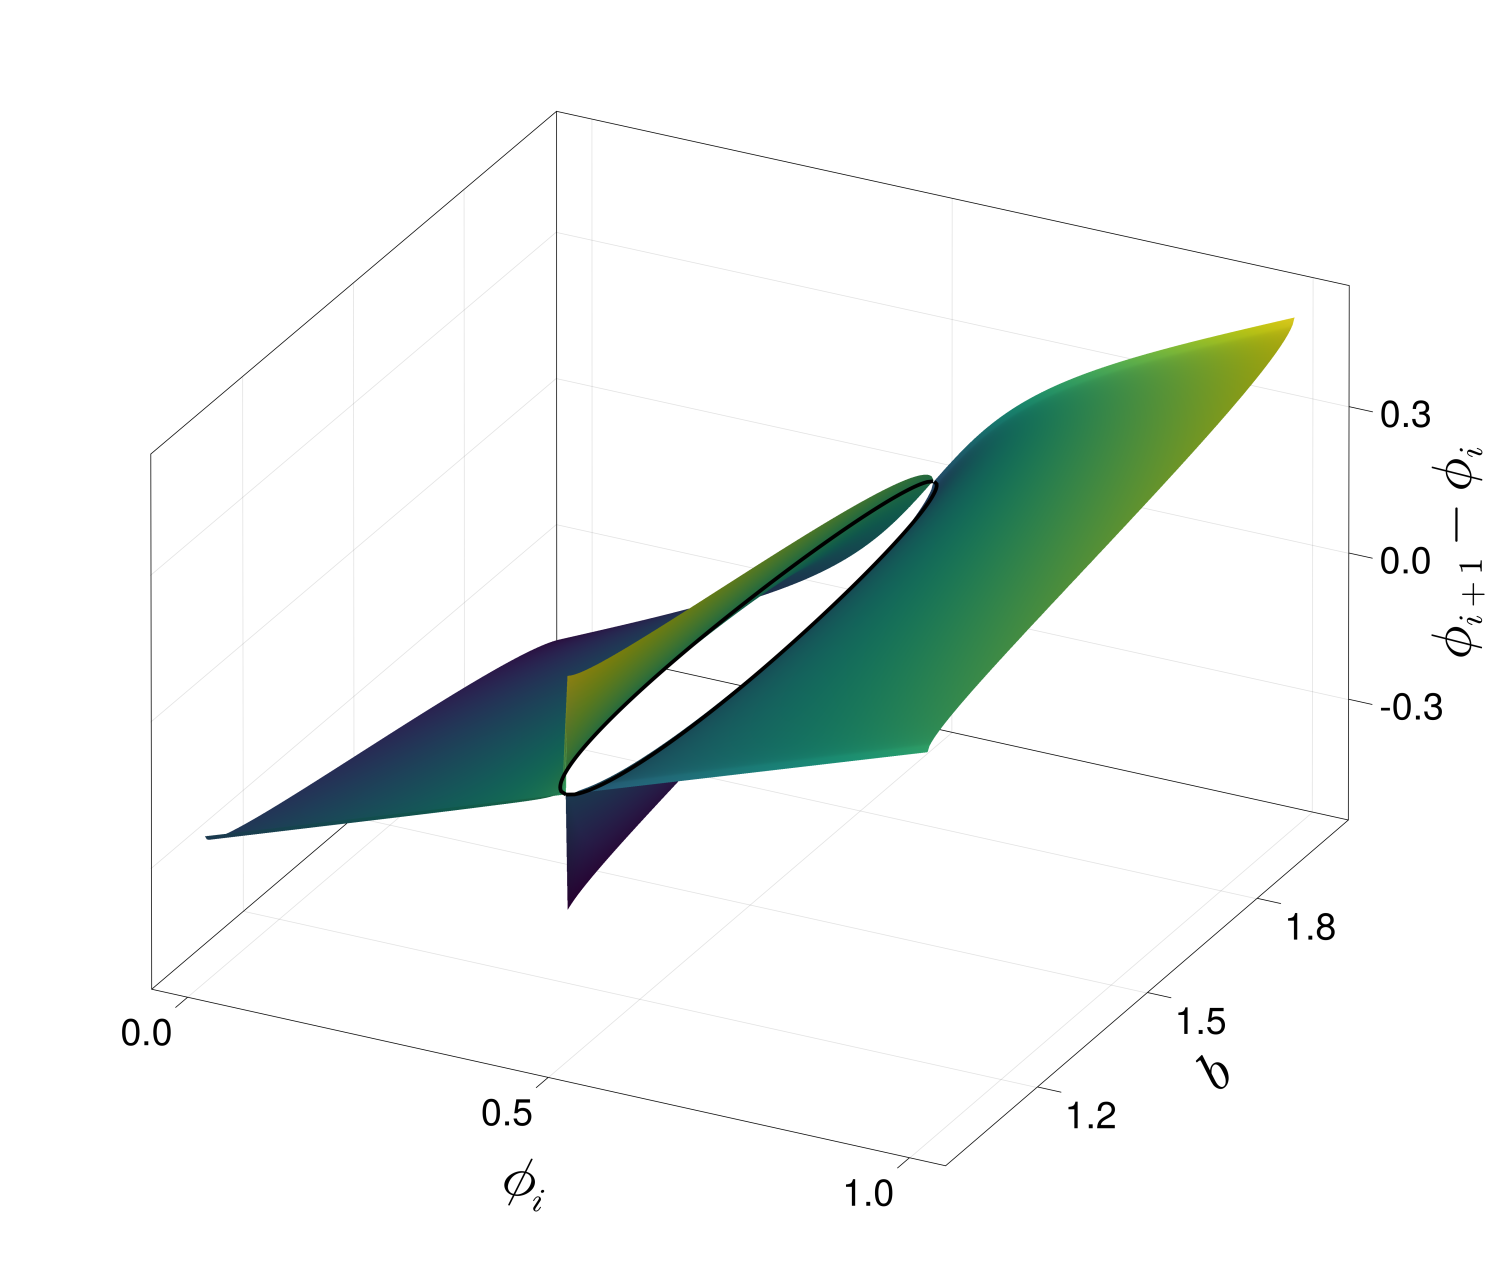
\includegraphics[width=.7\textwidth]{figures/eqs17_fig.png}
    \end{center}
\caption{The above surface is Eq.(\ref{eq: right}). The black line is Eq.(\ref{eq: square}) where $\phi_{i+1}=\phi_i$. Eq.(\ref{eq: right}) fully intersects Eq.(\ref{eq: square}) where the period-1 condition ($\phi_{i+1}=\phi_i$) is satisfied.}
\label{instabbound}
\end{figure}

\begin{figure}[H]
    \begin{center}
    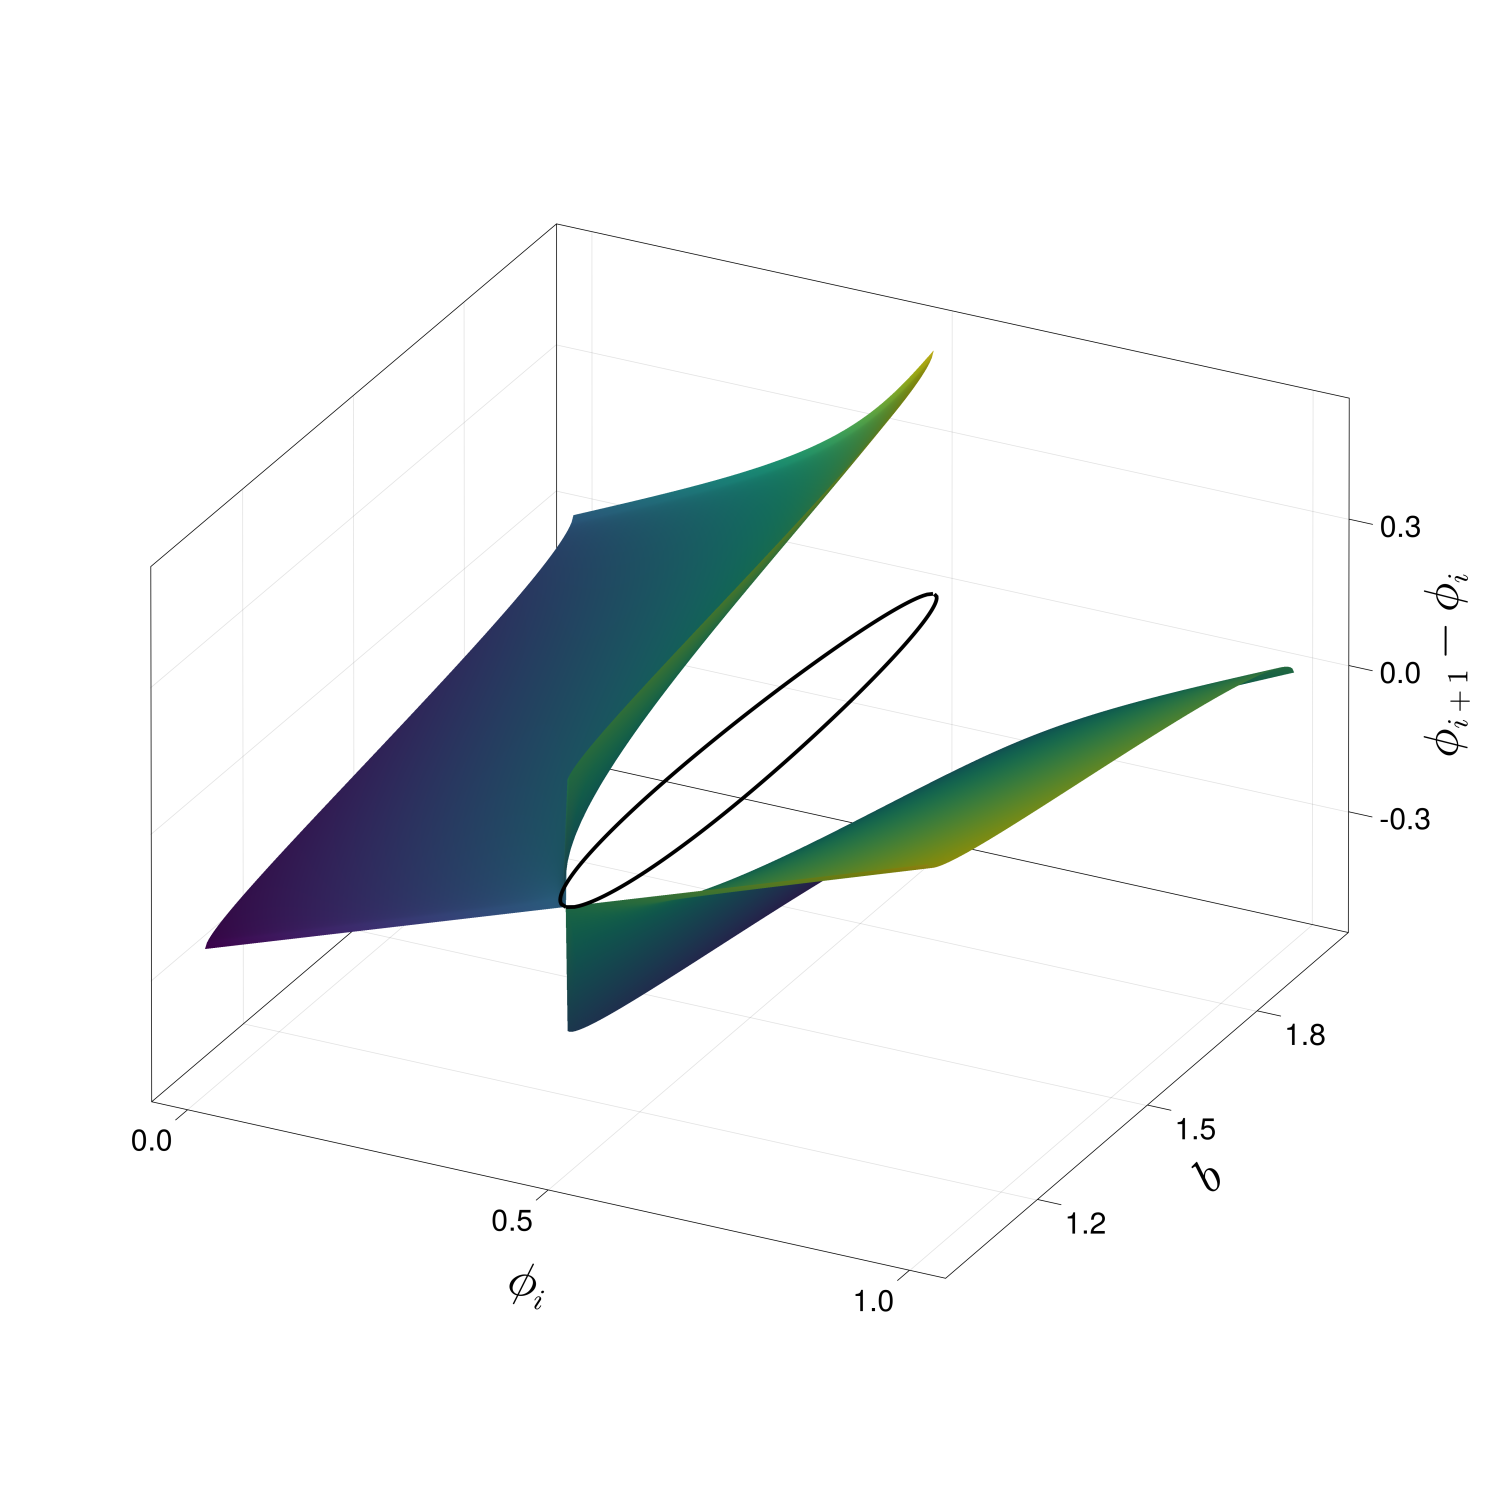
\includegraphics[width=.7\textwidth]{figures/eqs18_fig.png}
    \end{center}
    \caption{The above surface is Eq.(\ref{eq: wrong}). The black line is Eq.(\ref{eq: square}) where $\phi_{i+1}=\phi_i$. Eq.(\ref{eq: wrong}) does not intersect Eq.(\ref{eq: square}) anywhere the period-1 condition ($\phi_{i+1}=\phi_i$) is satisfied.}
    \label{instabbound_restric}
\end{figure}